\chapter{Data Selection and Analysis}

Every ALMA science project incorporates calibration observations of radio sources, which are mostly radio galaxies, to set various observational parameters of the science targets. These calibrations comprise the determination of bandpass, flux, and phase calibrations that lead to correct estimation of visibilities of the science targets. Therefore, multiple observations of ALMA calibrators must be made for each project.  

In this work, we will exploit the large amount of calibrators data acquired by ALMA, during its operation. By combining accumulated compatible data, we should be able to reach a sufficiently low noise level to obtain deep image to detect the environment of radio galaxies. Our target is to gather the maximum number of calibrators ($>20$) and make the deepest image so far in continuum for the ALMA bands available during the undertaking of this work. Some previous results have been demostrated in \cite{leon2016}.

The data are most likely acquired from Bands 3, 4, 6, 7, 8, and 9, accumulated from Cycle 1 to present. The data from Cycle 0 were not considered due to the use of smaller number of antennas during observations, leading to lower dynamic ranges. By automatizing at maximum the data reduction: downloading, self-calibration, concatenation, image ``cleaning'', and filtering, we should be able to study several radio galaxies in the range of redshift ($z$) from 0 to 2 with a very deep sensitivity of the order of a few tens of $\mu$Jy.


\section{Data Selection}
%\subsubsection{Selection Criteria}
To search for the calibrators utilized by ALMA to conduct their science programs, 
the ALMA Source Calibrator Catalogue (\url{https://almascience.eso.org/sc/}) is avalable and can be checked regularly. 
Subsequently, to obtain the corresponding data, one can access the ALMA Science Archive Query (\url{almascience.nrao.edu/aq}) 
to browse all the observations or projects 
that utilize the corresponding objects as calibrators. We have been using \textsf{astroquery.alma} to access and compile 
information from the ALMA Archive Database. 
For the first selection, we introduce specific criteria based only on the data availability, i.e., 
\begin{itemize}
\item Ignoring data from Cycle 0 due to the small number of antennas and the unfixed data structure
\item Neglecting polarization product and frequency resolution
\item Considering only observations using the 12m array 
\item Total integration time is sufficiently long, particularly in Bands 3, 6, and 7 
\item Publicly available data only 
\end{itemize}

\begin{table}
\caption{Selected ALMA calibrator based on data availability (query as of 10 April 2017).}
\begin{tabular}{lccccccccc}
\hline
Calibrator & $z$ & Flux (Jy) & \# projects & B3 & B4 & B6 & B7 & B8 & B9 \\
\hline
J0241-0815	&	0.005			&	1.003	&	22	&	1.1	&		&	1.8	&	3.5	&	0.5	&		\\
J0348-2749	&	0.991			&	0.73	&	23	&	1.1	&	0.3	&	1.8	&	2.8	&	0.1	&	0.1	\\
J0635-7516	&	0.653			&	1.41	&	25	&	1.3	&		&	3.1	&	1.1	&		&		\\
J0854+2006	&	0.3056			&	7.27	&	28	&	1.5	&	0.1	&	1.5	&	2.5	&		&	0.4	\\
J2253+1608	&	0.859			&	9.17	&	30	&	1.9	&	0.2	&	1.4	&	1	&	0.5	&	1.1	\\
J0006-0623	&	0.3467			&	4.163	&	32	&	1.4	&	0.2	&	1.1	&	2.9	&	0.4	&		\\
J1550+0527	&	1.422			&	0.97	&	34	&	2.8	&	0.3	&	2.1	&	2.6	&		&	0.8	\\
J1617-5848	&	1.422			&	1.11	&	35	&	4.6	&	0.2	&	1.9	&	1.9	&	0.1	&	0.1	\\
J2148+0657	&	0.99			&	1.6	&	41	&	1.2	&		&	3.5	&	3.6	&	1.1	&	0.5	\\
J2232+1143	&	1.037			&	6.29	&	43	&	1.9	&	0.2	&	1.1	&	3.5	&	1.8	&	0.4	\\
J0538-4405	&	0.894			&	1.98	&	46	&	2.2	&		&	3.8	&	2.9	&		&		\\
J0519-4546	&	0.035			&	1.27	&	47	&	3.9	&	0.7	&	4	&	1.6	&		&	0.1	\\
J0522-3627	&	0.0565			&	7.13	&	51	&	1.4	&		&	1.7	&	11.3	&	1	&	1.7	\\
J1337-1257	&	0.539			&	3.25	&	51	&	2.6	&	0.2	&	1.9	&	4.2	&		&	0.8	\\
J1229+0203	&	0.1583			&	10.05	&	57	&	3.3	&	0.5	&	4.5	&	3.7	&	0.5	&	0.8	\\
J1107-4449	&	1.598			&	1.06	&	58	&	3.4	&		&	4.1	&	1.3	&		&		\\
J1037-2934	&	0.312			&	2.28	&	59	&	1.6	&	0.6	&	3.6	&	3.3	&	0.1	&	0.5	\\
J1256-0547	&	0.5362			&	10.91	&	60	&	1.9	&	0.3	&	3.6	&	4.6	&	2.7	&	5.2	\\
J0238+1636	&	0.94			&	2.19	&	67	&	1.7	&	0.3	&	3.4	&	1.9	&	0.4	&		\\
J1517-2422	&	0.049			&	2.1	&	71	&	1.8	&	0.2	&	4.5	&	13.7	&	0.3	&	0.1	\\
J2258-2758	&	0.926			&	2.21	&	73	&	4.3	&	0.4	&	8	&	2.2	&	0.3	&	0.2	\\
J1427-4206	&	1.522			&	3.21	&	74	&	4.7	&		&	3.3	&	8.1	&	0.8	&	1.5	\\
J1058+0133	&	0.89			&	5.39	&	86	&	5	&	0.3	&	5.9	&	12.1	&	0.3	&	0.4	\\
J1924-2914	&	0.3526			&	5.6	&	87	&	2.7	&	0.4	&	5.5	&	11.9	&	2.1	&	2.3	\\
J1733-1304	&	0.902			&	2.91	&	87	&	4.6	&	0.7	&	12.4	&	6.2	&	0.1	&	0.3	\\
J0334-4008	&	1.445			&	0.9	&	103	&	8.2	&	2.9	&	10.2	&	4.9	&	0.4	&	1.6	\\
J0423-0120	&	0.9161			&	0.93	&	104	&	4.5	&	0.4	&	8.8	&	8.5	&	0.1	&	0.2	\\
\ldots	&	\ldots			&	\ldots	&	\ldots	&	\ldots	&	\ldots	&	\ldots	&	\ldots	&	\ldots	&	\ldots	\\
\hline
\end{tabular}
\label{tab:selectedcalibrator}
\noindent Notes: Columns B3 --- B9 are the total integration time (in hours) in the corresponding Bands 3 to 9, 
if we combine all the data from all the available projects. 
\end{table}

Based on these criteria, for example, if we require the total integration time longer than one hour for each Band 3, 6, 
and 7, then we can obtain 27 objects satisfying our requirement. Combining all of them, Table \ref{tab:selectedcalibrator}
presents the list of these 27 calibrators acquired from all the projects with the corresponding total integration time
(query as of 10 April 2017).
Redshifts ($z$) shown in Table \ref{tab:selectedcalibrator} are incorporated from  the NED website (NASA/IPAC {\it Extragalactic Database}, 
\url{http://ned.ipac.caltech.edu/forms/denv.html}). Flux in this table is taken from Band 3 and it may fluctuate significantly 
from days to weeks. \autoref{flowchart:dataselection} shows the detailed data selection process using a flowchart.

\begin{figure}[ht]
\centering
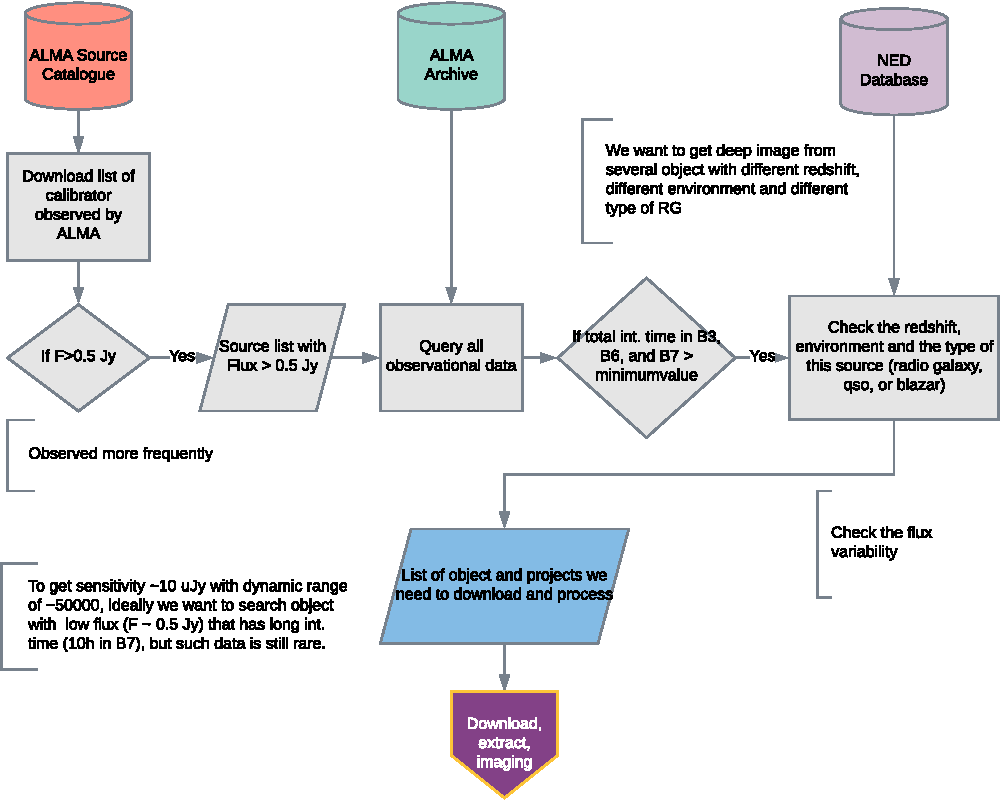
\includegraphics[width=\textwidth]{fig/selection-crop.pdf}
\caption{Flowchart of the data selection process.}
\label{flowchart:dataselection}
\end{figure}

For the second selection, concerning to study the environments of radio galaxies, we introduce further criteria 
for the objects based on their physical properties, i.e., (1) 
there are sources which are relatively isolated and other sources that are located in a group or clusters (in environment
of galaxies); and also (2) the selected samples should have different redshifts. However, such selection criteria are currently not 
applicable yet because of the still limited data available in public domain. 
Since the first goal of this research is to build a catalagoue or database of the point 
sources around the calibrators (radio galaxies), we apply the first selection criteria to retrieve the maximum number of
objects matching our criteria.  
Furthermore, considering our first results, we will conceive in-depth study from samples of radio galaxies based on 
the environment condition. We also envisage to write proposals of follow up observations following the results obtained.

%\subsubsection{Data Format and Limitation}

\section{Method}

Once the data are in public domain,  we can use these data from the ALMA archive through a selection process according to our defined science goals or constraints described above. However, care must be taken since every ALMA science project contains very big data. Typical data sizes from Cycle 1 and later are 25 -- 200 Gb for each science project before further processing (in tarred and zipped files). Sometimes, they are even bigger depending on the types of  the project, number of antenna, and time of integration. Data processing and further analyses will typically need more than 1 Tb disk size for one ALMA science project. Hence, one aspect of this work concerns about big data handling. We note that hundreds of ALMA science project will be selected during this work.

The {\it Common Astronomy Software Applications} package \citep[CASA, ][]{casa} is entirely used in this work to process the ALMA data. After downloading the raw data, we should perform the calibration from the ASDM file (ALMA Science Data Model) yielding
measurement set (MS) that is ready to process further. Generally, the final product is image as well as spectrum of the object. 

The data can be analyzed or processed individually and, subsequently, may be concatenated from several observations or bands. 
Note that one of the technical 
aspects in this work is to improve the dynamic range of the resulted image using wavelet filtering and detection of the 
point sources and absorption lines (different kernels) as well as to automatize the self-calibration. A first testbed was 
successfully applied to the calibrator PKS 0521-365, described in \cite{leon2016}.

\subsection{Splitting and Self-Calibration}

In details, we repeate the procedure here.
After selecting a calibrator, we can start by downloading the related project. Then, we split the data after converting it 
from ASDM to MS. For each project, usually there are three to four different objects observed as calibrators. Next, we collect 
all the calibrator data. Some of them 
may be used later since they were also selected in our source/calibrator list. Then the remaining data can be deleted to save the 
space disk. We remind that we deal with huge data.  

The splitted calibrator MS need to be self-calibrated. Self-calibration procedure is performed to increase the effective sensitivity 
of the image. This can be done by introducing a model of our source. We solve for the calibrations that best match 
our data to our model. We can get a model of our source through an initial image of our source. Self-calibration is 
recommended if the source have high enough signal-to-noise ratio (SNR), e.g., $> 20$ in our initial image. There are 
two types of self-calibration: phase (p) and amplitude-phase (ap). We already did some tests using our data and agreed 
to do three step of self-calibration, i.e. phase, phase, and then amplitude-phase calibration, to maximize the 
sensitivity or minimize the root-mean-square (rms) noise of the image ($\sigma$).

After self-calibration, we substract the image with a point source model in the location of calibrator. Substraction 
is done in the $uv$-plane, not in image plane. Substraction must be done to reduce the effect from the variability of 
the calibrator or central source to the (e.g. flux) environmental source that we want to extract and analyze. The whole procedure
is briefly shown in \autoref{fig:selfcal} using a flowchart. 

\begin{figure}[ht]
\centering
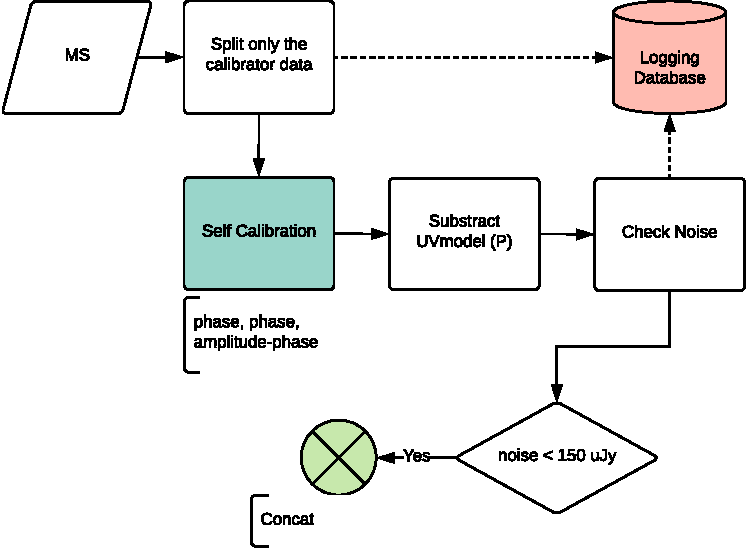
\includegraphics[width=0.8\textwidth]{fig/selfcal-crop.pdf}
\caption{Flowchart of collecting the calibrator data and self-calibration.}
\label{fig:selfcal}
\end{figure}

\subsection{Concatenating}

After collecting all the self-calibrated-substracted-MS of the calibrator, we can start to concatenate the data. 
Concatenating will increase the sensitivity of the final image. Each observation of a calibrator may only takes $3-6$ 
minutes, but if we can concatenate all the data from ALMA Archive, we can get a data with the total integration 
time up to several hours, without conducting a dedicated observation. It is worth noting that to concatenate image data, 
(1) we should not include bad data (after inspection, since they will not help to increase the SNR), 
(2) we can use a weighting based on the rms-noise of each initial images.

The pipeline to do the above processes have been developed, but some work has yet to be done to improve it. 
The example of point source that we 
successfully performed to extract the appropriate data using our pipeline is 
shown in \autoref{fig:test_J0241-0815_B7}. We notice that the detection of a very bright point 
source, at more than 10$\sigma$ level, can be identified at RA: $02^{h}41^{m}04.82^{s}$ and DEC: $-08^{\circ}15'15.0''$ (J2000) 
in northern part of the 
calibrator J0241-0815. This result is consistent with the similar work from ALMACAL team \citep{almacal1_2016}. 
We also detect a dim counterpart of that source in Band 3 and 6.

\begin{figure}[ht]
\centering
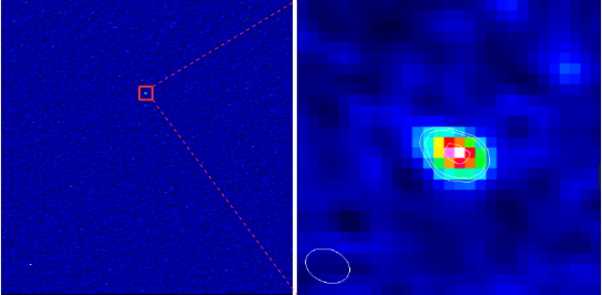
\includegraphics[width=\textwidth]{fig/J0241-0815_test.png}
\caption[First result of the workflow for the calibrator J0241-0815 in ALMA Band 7.]{Calibrator J0241-0815 in Band 7 (located at the center of left panel). We split this calibrator from the project, do self-calibration, subtract with a point source model, and then concat the resulted MSs. This image results from the combined data of 5 MSs, reducing the RMS noise level from $\sim$90 $\mu$Jy to 53 $\mu$Jy. We detect a point source in the the environment of this calibrator (see a zoom in feature in right panel). White contours represents $5\sigma$, $6\sigma$, and $10\sigma$ noise level, respectively.}
\label{fig:test_J0241-0815_B7}
\end{figure}

\section{Analysis}

To produce the catalogue of the point source emission in and around these radio galaxies from the final data/image, we will use a well-controlled image analysis software, e.g., SExtractor (\url{http://www.astromatic.net/software/sextractor}). The real point source may be identified in different frequencies/bands. This also can be used to produce the Spectral Energy Distribution (SED) of the source. If the source is not detected in all the bands, we need to be careful, since it might be either a real source or spurious data. Further analysis can be done by comparing the image with the observation from other range of electromagnetic observations, especially from other radio survey, optical, infrared, and X-ray. These additional data can be an image or a catalogue in the calibrator sky-region. Some related survey/archive that can be used such as SDSS, Hyper Suprime-Cam Subaru, MAST ( Multimission Archive at STScI), NED, Galex, Spitzer, WISE, and FIRST (Faint Images of the Radio Sky at Twenty-cm) survey. The corresponding information can be used to verify the point source detection and also to determine the SED of the object. It is important to check the quality of the final data/image by performing statistical tests, such as completeness test. We can also improve the dynamic range of the image using wavelet filtering.

The final output of the Ph.D thesis will be a very deep catalogue of the dust emission in and around radio galaxies to analyze the environment effects on the ISM content in these objects. This catalogue may include several parameters such as SED, spectral index, dust mass, and dust temperature. If the sample of calibrator/radio galaxy is large enough, we can see the effect of the galaxy evolution through the cosmic time (redshift) i.e. interplay between the activity of the central engine of radio galaxy (SMBH), star formation rates in the host galaxy, and the environment of the radio galaxy galaxy. The synchrotron emission (radio jets) with the high angular resolution will be analyzed, in particular its interaction with the dust in the host elliptical galaxies. We can measure the synchrotron emission using ALMA band 3, because the peak of this emission is in lower frequency (below 20 GHz), while the dust can be measure using ALMA band 6 and 7. 

The analysis of these data will be completed by the study of absorption lines towards the strong continuum of the radio galaxies to study the molecular gas content. These absorption lines in majority are expected from our own Galaxy, therefore this data will be important for mapping the molecular gas in our Galaxy.


\cleardoublepage
